\documentclass[11pt,a4paper]{article}

% --- Paquetes de Idioma y Tipografía ---
\usepackage[utf8]{inputenc}
\usepackage[spanish,es-tabla,es-noquoting]{babel}
\usepackage[T1]{fontenc}
\usepackage{lmodern}
\usepackage{microtype}

% --- Geometría y Márgenes ---
\usepackage[top=2.5cm, bottom=2.5cm, left=2.5cm, right=2.5cm, headheight=22pt]{geometry}

% --- Enlaces y Colores Sobrios Académicos ---
\usepackage{xcolor}
\definecolor{ugrRed}{RGB}{140, 20, 25}
\definecolor{etsiitBlue}{RGB}{20, 50, 95}
\definecolor{darkGray}{RGB}{40, 45, 50}
\definecolor{codeBg}{RGB}{248, 249, 250}
\definecolor{codeFrame}{RGB}{210, 215, 220}

\usepackage[colorlinks=true, linkcolor=etsiitBlue, urlcolor=etsiitBlue, citecolor=ugrRed]{hyperref}

% --- Paquetes Matemáticos y Tablas ---
\usepackage{amsmath, amssymb}
\usepackage{booktabs}
\usepackage{tabularx}
\usepackage{array}
\usepackage{tikz}
\usetikzlibrary{shapes.geometric, arrows.meta, positioning, calc}
\usepackage{graphicx}
\usepackage{caption}
\usepackage{subcaption}

% --- Formato de Listados de Código ---
\usepackage{listings}
\lstset{
    backgroundcolor=\color{codeBg},
    basicstyle=\ttfamily\footnotesize,
    keywordstyle=\color{etsiitBlue}\bfseries,
    commentstyle=\color{gray}\itshape,
    stringstyle=\color{ugrRed},
    breaklines=true,
    breakatwhitespace=true,
    tabsize=2,
    frame=single,
    rulecolor=\color{codeFrame},
    captionpos=b,
    showstringspaces=false
}

% --- Formato de Títulos y Encabezados ---
\usepackage{titlesec}
\titleformat{\section}{\Large\bfseries\color{etsiitBlue}}{\thesection}{1em}{}[\titlerule]
\titleformat{\subsection}{\large\bfseries\color{etsiitBlue!90}}{\thesubsection}{0.8em}{}
\titleformat{\subsubsection}{\normalsize\bfseries\color{ugrRed}}{\thesubsubsection}{0.6em}{}

\usepackage{fancyhdr}
\pagestyle{fancy}
\fancyhf{}
\fancyhead[L]{\small \textit{NPI - Punto de Información Multimodal ETSIIT}}
\fancyhead[R]{\small \textit{Memoria Técnica del Software}}
\fancyfoot[C]{\thepage}
\renewcommand{\headrulewidth}{0.4pt}

\begin{document}

% =========================================================================
% PORTADA TÉCNICA
% =========================================================================
\begin{titlepage}
    \centering
    \vspace*{0.4cm}
    \IfFileExists{doc/memoria/images/logo-ugr-grande.png}{%
        \includegraphics[width=0.42\textwidth]{doc/memoria/images/logo-ugr-grande.png}%
    }{\IfFileExists{images/logo-ugr-grande.png}{%
        \includegraphics[width=0.42\textwidth]{images/logo-ugr-grande.png}%
    }{}}\par
    \vspace{0.8cm}
    {\scshape\Large Universidad de Granada \par}
    \vspace{0.2cm}
    {\scshape\large Escuela Técnica Superior de Ingenierías Informática y de Telecomunicación \par}
    \vspace{0.2cm}
    {\normalsize Grado en Ingeniería Informática --- 4º Curso \par}
    \vspace{0.1cm}
    {\normalsize Asignatura: Nuevos Paradigmas de Interacción (NPI) \par}

    \vspace{1.0cm}
    \hrule height 1.5pt
    
    \vspace{0.4cm}
    {\huge \bfseries Memoria Técnica del Software \par}
    \vspace{0.3cm}
    {\Large \bfseries Sistema de Punto de Información Multimodal, Ubicuo y Accesible para la ETSIIT \par}
    \vspace{0.4cm}
    \hrule height 0.8pt

    \vspace{1.2cm}
    \begin{minipage}{0.85\textwidth}
        \textbf{Equipo de Desarrollo (Grupo):}
        \vspace{0.3cm}
        \begin{itemize}
            \item \textbf{Ángela Rodríguez} --- \texttt{angelarodr15@correo.ugr.es}
            \item \textbf{Laura Sanz Lobo} --- \texttt{laurasanzlobo@correo.ugr.es}
            \item \textbf{José Pedregosa} --- \texttt{josepc@correo.ugr.es}
        \end{itemize}
    \end{minipage}

    \vfill
    {\normalsize Convocatoria Ordinaria --- Curso Académico 2026/2027 \par}
    {\normalsize Granada, a \today \par}
\end{titlepage}

% =========================================================================
% RESUMEN Y CONTENIDOS
% =========================================================================
\pagenumbering{roman}

\begin{abstract}
\noindent En este documento se presenta la memoria técnica exhaustiva del software desarrollado para el Punto de Información de la ETSIIT - UGR. El documento describe en profundidad la totalidad de clases, variables miembro, algoritmos, métodos públicos y bibliotecas externas involucradas. 

Se desglosa la ingeniería de interacción gestual en mano basada en acelerometría y gravedad con resolución del problema de Midas (retorno al campo de visión y discriminación temporal estricta); el motor fonético y semántico de procesamiento en lenguaje natural para consultas por voz; el sistema de visión artificial y sensores físicos para autenticación del estudiante (cámara con Google ML Kit Barcode y OCR, y lector NFC); el algoritmo de Dijkstra implementado sobre un grafo completo de 306 nodos y 333 aristas que cubre las 6 plantas de la facultad con soporte para rutas rápidas y accesibles en silla de ruedas; y el subsistema de geoposicionamiento y enrutamiento peatonal hacia comedores universitarios.
\end{abstract}

\vspace{0.8cm}
\tableofcontents
\newpage
\pagenumbering{arabic}

% =========================================================================
\section{Introducción y Objetivos del Sistema}
% =========================================================================

\subsection{Contextualización y Problemática}
Los quioscos o puntos de información habituales en los edificios universitarios suelen presentar una arquitectura rígida: pantallas táctiles fijas situadas en el vestíbulo o aplicaciones móviles que replican los portales web con extensas listas de navegación jerárquica. Este diseño presenta graves inconvenientes:
\begin{enumerate}
    \item \textbf{Falta de accesibilidad y esfuerzo cognitivo:} Exige a los estudiantes o visitantes con prisas detenerse a teclear nombres en pantallas públicas o navegar por menús complejos para saber si un profesor está en su despacho o en qué aula se imparte una clase.
    \item \textbf{Ausencia de sensibilidad al contexto temporal (\textit{Context-Awareness}):} Las fichas de los profesores suelen mostrar estáticamente los horarios de tutorías y docencia sin evaluar si el instante actual coincide con alguna de esas franjas, delegando el cálculo mental en el usuario.
    \item \textbf{Dependencia de la interacción táctil estricta:} En situaciones de desplazamiento activo por pasillos, la interacción mediante botones pequeños resulta incómoda e insegura.
\end{enumerate}

\subsection{Objetivos Técnicos}
El software desarrollado tiene como meta implementar un \textbf{asistente ubicuo y multimodal} que supere estas barreras mediante:
\begin{itemize}
    \item Captura de intenciones por múltiples canales independientes: voz natural en español (reconocimiento y síntesis fonética), gestos físicos en mano evaluados mediante acelerometría y vector de gravedad, y toques táctiles.
    \item Evaluación contextual en tiempo real del horario del estudiante y de los 35 profesores clave de la facultad.
    \item Guiado topológico integral: navegación exterior por GPS con OpenRouteService hacia los comedores del campus y handoff transparente al mapa interior de 6 plantas mediante el algoritmo de Dijkstra.
    \item Autenticación mediante credenciales físicas universitarias combinando cámara (código QR y OCR del carnet TUI) con lectura de chips NFC.
\end{itemize}

% =========================================================================
\section{Bibliotecas Externas y Dependencias Incorporadas}
% =========================================================================

En la Tabla~\ref{tab:librerias} se desglosan en detalle las bibliotecas y SDKs externos integrados en el archivo \texttt{build.gradle.kts}, analizando su papel en el sistema y los motivos técnicos de su elección.

\begin{table}[ht!]
\centering
\small
\renewcommand{\arraystretch}{1.2}
\begin{tabularx}{\textwidth}{l p{3.6cm} X}
\toprule
\textbf{Biblioteca / SDK} & \textbf{Identificador / Versión} & \textbf{Justificación y Función Técnica} \\
\midrule
\textbf{Jetpack Compose BOM} & \texttt{androidx.compose.bom} & Motor declarativo de UI. Facilita la reactividad del estado de sesión (\texttt{UserSessionRepository}) y el renderizado eficiente de animaciones (pulsos de tutoría, barras de progreso temporal). \\
\textbf{Play Services Location} & \texttt{21.3.0} & Acceso optimizado al hardware GPS del dispositivo mediante \texttt{FusedLocationProviderClient}. Aplica filtros de precisión balanceando el consumo de batería durante la navegación exterior. \\
\textbf{MapLibre GL Android} & \texttt{org.maplibre.gl:13.7.1} & Motor de renderizado vectorial open-source. Permite dibujar cartografía y polilíneas peatonales GeoJSON sin depender de cuotas ni licencias privativas de Google Maps SDK. \\
\textbf{OpenRouteService API} & Cliente REST nativo & Motor de enrutamiento a pie (\texttt{foot-walking}). Devuelve coordenadas geográficas precisas sobre la red de aceras para trazar el camino a los comedores universitarios. \\
\textbf{Google ML Kit Barcode} & \texttt{17.3.0} & Reconocimiento local por visión artificial de códigos QR de la TUI en tiempo real a 30 FPS sin enviar fotogramas a servidores externos. \\
\textbf{Google ML Kit Text} & \texttt{16.0.1} & Motor de OCR en dispositivo para escanear y validar el DNI y nombre del alumno impresos sobre la tarjeta física. \\
\textbf{Google Gson} & \texttt{2.10.1} & Serialización y deserialización de las estructuras JSON complejas (\texttt{grafo\_etsiit\_completo.json}, \texttt{docentes.json} y persistencia de sesión). \\
\textbf{Android TTS \& Speech} & \texttt{android.speech} nativo & Síntesis de voz en español (\texttt{TextToSpeech}) y reconocimiento acústico de voz (\texttt{RecognizerIntent}) para diálogo bidireccional. \\
\bottomrule
\end{tabularx}
\caption{Bibliotecas externas y SDKs incorporados en el proyecto.}
\label{tab:librerias}
\end{table}

% =========================================================================
\section{Diagramas del Sistema}
% =========================================================================

\subsection{Diagrama de Arquitectura Modular por Capas}
En la Figura~\ref{fig:arquitectura} se ilustra la arquitectura desacoplada del sistema, organizada en cuatro niveles: Hardware Físico, Controladores de Sensores, Lógica de Dominio y Capa de Presentación Reactiva (Compose).

\begin{figure}[ht!]
\centering
\begin{tikzpicture}[
    box/.style={rectangle, draw=etsiitBlue, fill=white, rounded corners=2pt, thick, align=center, text width=3.4cm, minimum height=1.1cm, font=\footnotesize},
    sensorBox/.style={rectangle, draw=ugrRed, fill=white, rounded corners=2pt, thick, align=center, text width=3.4cm, minimum height=1.1cm, font=\footnotesize},
    arrow/.style={-{Stealth[length=2.5mm]}, thick, draw=black!70}
]

% Nivel 1: Hardware
\node[sensorBox] (acc) at (0, 6) {\textbf{Sensores Inerciales}\\\textit{Acelerómetro + Gravedad}};
\node[sensorBox] (gps) at (4.8, 6) {\textbf{Antena GPS / GNSS}\\\textit{FusedLocationProvider}};
\node[sensorBox] (cam) at (9.6, 6) {\textbf{Cámara Camera2 / NFC}\\\textit{Captura óptica y chip}};

% Nivel 2: Gestores de Sensores
\node[box] (accMgr) at (0, 4) {\textbf{AccelerometerManager}\\\textit{TripleTilt, Twist, Lifted}};
\node[box] (gpsRdr) at (4.8, 4) {\textbf{GpsLocationReader}\\\textit{StateFlow<Location?>}};
\node[box] (ocrScn) at (9.6, 4) {\textbf{TuiOcrScanner}\\\textit{ML Kit QR + OCR}};

% Nivel 3: Dominio / Lógica
\node[box] (grafo) at (1.5, 2) {\textbf{GrafoETSIIT}\\\textit{Dijkstra + Fonética Voz}};
\node[box] (outNav) at (5.5, 2) {\textbf{OutdoorNavigator}\\\textit{ORS + Haversine Arrival}};
\node[box] (userRepo) at (9.6, 2) {\textbf{UserSessionRepository}\\\textit{StateFlow Perfil y Matrícula}};

% Nivel 4: Capa de Presentación UI
\node[box] (navScr) at (1.5, 0) {\textbf{NavigationScreen}\\\textit{Plano 2D / Guiado Vertical}};
\node[box] (profScr) at (5.5, 0) {\textbf{ProfessorsScreen}\\\textit{Docentes, TTS, Intent Correo}};
\node[box] (profProfile) at (9.6, 0) {\textbf{ProfileScreen / Home}\\\textit{Horario y Estado Sesión}};

% Enlaces
\draw[arrow] (acc) -- (accMgr);
\draw[arrow] (gps) -- (gpsRdr);
\draw[arrow] (cam) -- (ocrScn);

\draw[arrow] (accMgr) -- (navScr);
\draw[arrow] (accMgr) -- (profScr);
\draw[arrow] (gpsRdr) -- (outNav);
\draw[arrow] (ocrScn) -- (userRepo);

\draw[arrow] (grafo) -- (navScr);
\draw[arrow] (outNav) -- (navScr);
\draw[arrow] (userRepo) -- (profScr);
\draw[arrow] (userRepo) -- (profProfile);

\end{tikzpicture}
\caption{Diagrama de arquitectura modular por capas del software.}
\label{fig:arquitectura}
\end{figure}

\subsection{Diagrama de Estados: Detección Gestual con Retorno a Línea de Visión}
La Figura~\ref{fig:estados_nod} muestra la máquina de estados finitos que gobierna la ejecución de acciones gestuales. Se observa cómo el sistema exige que el vector de aceleración regrese a la región de lectura antes de confirmar la orden, evitando disparos involuntarios.

\begin{figure}[ht!]
\centering
\begin{tikzpicture}[
    state/.style={ellipse, draw=etsiitBlue, fill=white, thick, minimum width=2.6cm, align=center, font=\footnotesize},
    arrow/.style={-{Stealth[length=2.5mm]}, thick, draw=black!80}
]

\node[state] (idle) at (0, 0) {\textbf{IDLE}\\\textit{Móvil inclinado}\\$Z \ge 3.8\text{ m/s}^2$};
\node[state] (down) at (4.5, 0) {\textbf{VERTICAL / TILT}\\\textit{Acción gestual}\\$Z \le 2.1, Y \ge 8.1$};
\node[state] (back) at (9, 0) {\textbf{RETORNO A BASE}\\\textit{Línea de visión}\\$Z \ge 3.8\text{ m/s}^2$};
\node[state, draw=ugrRed] (action) at (9, -2.4) {\textbf{CONFIRMACIÓN}\\\textit{Diálogo 1.8s + Vibración}};

\draw[arrow] (idle) -- node[above, font=\scriptsize] {Desplazamiento angular} (down);
\draw[arrow] (down) -- node[above, font=\scriptsize] {Vuelta a posición inicial} (back);
\draw[arrow] (back) -- node[right, font=\scriptsize] {Gesto completado} (action);
\draw[arrow] (down.south) to[bend left=30] node[below, font=\scriptsize] {Timeout $> 2.2$\,s (movimiento abortado)} (idle.south);
\draw[arrow] (action.west) to[bend left=20] node[below, font=\scriptsize] {Disparo de Intent o Navegación} (idle.south);

\end{tikzpicture}
\caption{Autómata de estados finitos para la confirmación gestual en mano con retorno a línea de visión.}
\label{fig:estados_nod}
\end{figure}

% =========================================================================
\section{Descripción Detallada del Software}
% =========================================================================

En esta sección se describen minuciosamente las clases, variables miembro y métodos públicos de cada uno de los subsistemas de la aplicación.

% -------------------------------------------------------------------------
\subsection{Paquete de Sensores y Gestos (\texttt{com.example.npi\_puntoinfo\_etsiit.sensors})}

\subsubsection{Clase \texttt{AccelerometerManager}}
Constituye el controlador central del hardware inercial del terminal. Implementa la interfaz \texttt{SensorEventListener} de Android y se encarga de discriminar cuatro gestos distintos:

\begin{enumerate}
    \item \textbf{Gesto de Clase Actual (3 inclinaciones rápidas hacia adelante y vuelta):}
    Detecta 3 cabeceos consecutivos en un intervalo temporal estricto menor a 1.6 segundos (máximo 600\,ms entre cabeceos). Si el usuario tarda más, el contador se resetea a cero para evitar falsos positivos acumulados al caminar.
    \item \textbf{Gesto <<¡Llévame!>> (Inclinación a la izquierda y retorno):}
    Giro del móvil hasta que la aceleración lateral supere $X \ge 7.5\text{ m/s}^2$ durante al menos 80\,ms y retorno a la posición neutra ($X \le 2.4\text{ m/s}^2$) en menos de 2.4 segundos.
    \item \textbf{Gesto de Acción Rápida (Correo / Reserva de Comedor):}
    Partiendo de la postura inclinada de lectura ($Z \ge 3.8\text{ m/s}^2$), el usuario lleva el móvil a vertical frente a sí ($Z \le 2.1\text{ m/s}^2, Y \ge 8.1\text{ m/s}^2$) y lo devuelve a la posición inclinada inicial.
    \item \textbf{Gesto de Guiado Vertical (Levantamiento de Navegación):}
    Mantenimiento del terminal en vertical estricto frente a los ojos para conmutar al guiado paso a paso con fotos, o retorno a posición horizontal para ver el mapa 2D.
\end{enumerate}

\paragraph{Variables miembro y constantes de calibración:}
\begin{itemize}
    \item \texttt{sensorManager: SensorManager?}: Acceso al servicio nativo de sensores.
    \item \texttt{accelerometer: Sensor?}, \texttt{gyroscope: Sensor?}: Descriptores de hardware inercial.
    \item \texttt{tripleForwardTiltDetector: TripleForwardTiltDetector}: Objeto interno que mantiene el estado y la ventana temporal de los 3 cabeceos consecutivos.
    \item \texttt{TILT\_LEFT\_STRONG\_THRESHOLD = 7.5f}: Umbral en el eje $X$ para detectar el giro de muñeca a la izquierda.
    \item \texttt{RETURN\_NEUTRAL\_MAX\_X = 2.4f}: Umbral de histéresis para confirmar el regreso a la posición base en el eje $X$.
    \item \texttt{INCLINED\_MIN\_Z = 3.8f}, \texttt{VERTICAL\_MAX\_Z\_FOR\_ACTION = 2.1f}: Umbrales en el eje $Z$ para detectar la transición entre postura inclinada de lectura y vertical.
    \item \texttt{VERTICAL\_MIN\_Y\_FOR\_ACTION = 8.1f}: Umbral en el eje $Y$ para verificar la posición vertical del teléfono.
    \item \texttt{MAX\_VERTICAL\_ACTION\_WINDOW\_MS = 2200L}: Ventana máxima para completar el ciclo de ida y vuelta.
    \item \textbf{Callbacks expuestos:}
    \begin{itemize}
        \item \texttt{var onShakeDetected: (() -> Unit)?}: Disparado tras 3 cabeceos completos para mostrar la clase actual.
        \item \texttt{var onTakeMeThereGesture: (() -> Unit)?}: Disparado tras el giro de muñeca para iniciar ruta.
        \item \texttt{var onNodStarted: (() -> Unit)?}: Disparado al detectar la primera fase de inclinación hacia vertical.
        \item \texttt{var onForwardTiltGesture: (() -> Unit)?}: Disparado al completarse el retorno a la posición de lectura.
        \item \texttt{var onPostureModeChanged: ((isVertical: Boolean) -> Unit)?}: Notifica si el móvil se sostiene horizontal o verticalmente para alternar entre el mapa 2D y el guiado de navegación.
    \end{itemize}
\end{itemize}

\paragraph{Métodos principales:}
\begin{itemize}
    \item \texttt{fun startListening()}: Registra los escuchadores del acelerómetro con frecuencia \texttt{SENSOR\_DELAY\_GAME} (aproximadamente 50\,Hz) para garantizar respuesta en tiempo real sin latencia perceptible.
    \item \texttt{fun stopListening()}: Desvincula los listeners para evitar consumo residual de batería en segundo plano.
    \item \texttt{fun onSensorChanged(event: SensorEvent)}: Ejecuta el procesamiento de señal en cada muestra. Clasifica el vector en \texttt{DeviceOrientation} (\texttt{VERTICAL}, \texttt{FLAT}, \texttt{TILTED\_LEFT}, \texttt{TILTED\_RIGHT}) y evalúa los temporizadores de histéresis de cada gesto.
\end{itemize}

\subsubsection{Clase \texttt{ProximityManager}}
Supervisa el sensor de proximidad frontal (\texttt{Sensor.TYPE\_PROXIMITY}) situado junto al auricular del teléfono. Incorpora un mecanismo de filtrado temporal de 350\,ms para evitar que el paso fugaz de una mano active falsamente la acción. Expone el callback \texttt{onDeviceCovered: (() -> Unit)?} utilizado para confirmaciones silenciosas y apagado de alertas de voz.

\subsubsection{Clase \texttt{GpsLocationReader} y \texttt{DeviceLocationProvider}}
Gestionan la suscripción al proveedor de localización satelital (\texttt{FusedLocationProviderClient}) mediante la biblioteca de Google Play Services. Emite una secuencia reactiva \texttt{locationFlow: StateFlow<Location?>} que informa a la aplicación de cambios en latitud, longitud, velocidad y precisión estimada en metros.

% -------------------------------------------------------------------------
\subsection{Motor Topológico Interior y Algoritmo Dijkstra (\texttt{GrafoETSIIT.kt})}

\subsubsection{Modelos de Datos Topológicos}
La representación matemática del edificio se modela mediante las siguientes clases de datos:
\begin{itemize}
    \item \texttt{data class Nodo(id: String, nombre: String, planta: String, edificio: String, tipo: String, x: Int, y: Int)}: Representa un punto de interés o una intersección de pasillos. Los tipos admitidos son: \texttt{"despacho"}, \texttt{"aula"}, \texttt{"laboratorio"}, \texttt{"escalera"}, \texttt{"ascensor"}, \texttt{"servicio"}, \texttt{"acceso"}, \texttt{"pasillo"}. Las coordenadas $(x, y)$ se corresponden con la posición gráfica sobre el plano de planta de la facultad.
    \item \texttt{data class AristaJson(origen: String, destino: String, distancia\_metros: Int)}: Representa el segmento transitable entre dos nodos y su longitud real en metros.
    \item \texttt{data class RutaCalculada(origen: Nodo, destino: Nodo, nodos: List<Nodo>, distanciaMetros: Int, tiempoEstimadoSegundos: Int)}: Objeto que agrupa el camino de coste mínimo resuelto, calculando además una estimación de tiempo a velocidad peatonal media ($1.2\text{ m/s}$).
\end{itemize}

\subsubsection{Clase \texttt{GrafoETSIIT}}
Alberga las estructuras de datos del grafo y la lógica algorítmica de cálculo de caminos y reconocimiento de voz:

\paragraph{Variables miembro:}
\begin{itemize}
    \item \texttt{directorioNodos = mutableMapOf<String, Nodo>()}: Diccionario hash que permite recuperar cualquier nodo por su identificador en tiempo constante $O(1)$. Contiene 306 nodos.
    \item \texttt{conexiones = mutableMapOf<String, MutableList<AristaDijkstra>>()}: Lista de adyacencia no dirigida indexada por ID de nodo origen, almacenando el ID destino y la distancia ponderada. Contiene 333 aristas.
\end{itemize}

\paragraph{Métodos principales:}
\begin{itemize}
    \item \texttt{fun cargarDesdeAssets(context: Context, nombreArchivo: String)}: Deserializa el JSON del grafo en memoria y construye la lista de adyacencia bidireccional.
    \item \texttt{fun calcularRutaDijkstra(origenId: String, destinoId: String, soloAccesible: Boolean = false): List<Nodo>}: 
    Implementación del algoritmo de caminos mínimos de Dijkstra mediante cola de prioridad (\texttt{PriorityQueue<Pair<Int, String>>}). Opera con una complejidad temporal de $O((|V| + |E|) \log |V|)$. Si el parámetro \texttt{soloAccesible} es verdadero (modo silla de ruedas / movilidad reducida), el algoritmo filtra y descarta las aristas que conectan con nodos de tipo \texttt{"escalera"}, forzando el camino a través de los núcleos de ascensores (\texttt{"ascensor"}).
    \item \texttt{fun resolverDestinoPorVoz(texto: String): ResultadoVoz}: 
    Analizador fonético y semántico que resuelve consultas dictadas por voz en español:
    \begin{enumerate}
        \item Normaliza tildes y caracteres especiales mediante eliminación diacrítica NFD.
        \item Normaliza números hablados complejos (\textit{"cuatrocientos veinte"} $\rightarrow$ \texttt{"420"}, \textit{"treinta y cinco"} $\rightarrow$ \texttt{"35"}).
        \item Discrimina consultas de despachos docentes frente a aulas y laboratorios (ej. diferencia \textit{"aula 3.4"} de un despacho).
        \item Mapea nombres de profesores y servicios comunes (\textit{"comedor"}, \textit{"cafetería"}, \textit{"secretaría"}) a sus correspondientes nodos físicos en el grafo.
    \end{enumerate}
\end{itemize}

% -------------------------------------------------------------------------
\subsection{Navegación Exterior y Geovalla (\texttt{outdoor})}

\subsubsection{Clase \texttt{OutdoorNavigator}}
Orquesta la consulta y presentación de rutas peatonales en el exterior del campus:
\begin{itemize}
    \item \textbf{Atributos:} \texttt{gpsReader: GpsLocationReader}, \texttt{orsClient: OpenRouteService}, \texttt{state: StateFlow<OutdoorState>}.
    \item \textbf{Métodos:} \texttt{setDestination(destinationId: String)}, \texttt{recalculateRoute()}. Conecta de forma asíncrona mediante corrutinas de Kotlin con la API de OpenRouteService, procesa la respuesta GeoJSON y genera la lista de instrucciones de giro (\texttt{WalkingStep}).
\end{itemize}

\subsubsection{Clase \texttt{ArrivalDetector}}
Implementa el algoritmo de detección de llegada a la ETSIIT mediante la ecuación esférica de Haversine:
\begin{equation}
d = 2 R \cdot \arcsin\left(\sqrt{\sin^2\left(\frac{\Delta \phi}{2}\right) + \cos(\phi_1)\cos(\phi_2)\sin^2\left(\frac{\Delta \lambda}{2}\right)}\right)
\end{equation}
Donde $R = 6371\text{ km}$ representa el radio terrestre medio, $\phi$ la latitud y $\lambda$ la longitud. Si la distancia actual $d \le 25\text{ metros}$ respecto a la puerta exterior de la ETSIIT ($37.19705^\circ\text{ N}, -3.62452^\circ\text{ W}$), la clase activa el evento de llegada para invitar al usuario a transicionar al mapa interior de plantas.

% -------------------------------------------------------------------------
\subsection{Autenticación, Sesión y Visión Artificial (\texttt{data} y \texttt{ocr})}

\subsubsection{Objeto \texttt{UserSessionRepository}}
Singleton reactivo encargado de la persistencia y control de la sesión del estudiante:
\begin{itemize}
    \item \textbf{Variables miembro:}
    \begin{itemize}
        \item \texttt{currentProfileState: MutableState<UserProfile?>}: Estado observable por Jetpack Compose para desencadenar la recomposición inmediata de la interfaz al iniciar o cerrar sesión.
        \item \texttt{officialMatricula: Map<String, String>}: Asignaturas matriculadas del curso (NPI, VC, PL, PTC, SS, TIC) con sus correspondientes subgrupos prácticos.
    \end{itemize}
    \item \textbf{Métodos principales:}
    \begin{itemize}
        \item \texttt{fun getProfile(context: Context): UserProfile}: Recupera el perfil almacenado en \texttt{SharedPreferences} con verificación de integridad de datos.
        \item \texttt{fun loginWithOfficialProfile(context: Context, isAccessibleRouting: Boolean): UserProfile}: Inicia sesión tras la lectura biométrica/TUI asignando el perfil de estudiante.
        \item \texttt{fun logout(context: Context)}: Limpia la sesión y devuelve la aplicación a su estado genérico para visitantes.
    \end{itemize}
\end{itemize}

\subsubsection{Clase \texttt{TuiOcrScanner}}
Controlador de visión por computador basado en la API Camera2 de Android:
\begin{itemize}
    \item Canaliza los fotogramas del sensor de la cámara en paralelo hacia dos pipelines independientes de Google ML Kit:
    \begin{enumerate}
        \item \texttt{BarcodeScanning}: Decodifica el código QR de la TUI Universitaria.
        \item \texttt{TextRecognition}: Aplica OCR sobre el texto plano para extraer y validar el formato del DNI español (8 dígitos y letra de control) y el nombre del titular impreso.
    \end{enumerate}
\end{itemize}

\subsubsection{Clase \texttt{NfcCardReader}}
Gestiona la antena NFC en modo \textit{Foreground Dispatch}. Intercepta tags de tipo Mifare Classic y Ultralight presentes en la tarjeta física universitaria para autenticar al usuario por contacto físico directo en el reverso del terminal.

% -------------------------------------------------------------------------
\subsection{Capa de Presentación e Interfaz (\texttt{ui.screens})}

\subsubsection{Componente Composable \texttt{ProfessorsScreen}}
Pantalla que implementa el catálogo de 35 docentes universitarios:
\begin{itemize}
    \item \textbf{Cálculo de actividad en tiempo real (\texttt{getProfessorActivityStatus}):} Evalúa la hora del sistema (o la hora simulada en el menú demo) cruzándola con los campos \texttt{"tutorias"} y \texttt{"clases"} del JSON docente. Determina el estado: \texttt{IN\_OFFICE\_HOURS} (en tutoría con punto pulsante \texttt{StatusDot}), \texttt{IN\_CLASS} (en clase indicando el aula actual) o \texttt{OFFLINE} (fuera de horario).
    \item \textbf{Síntesis de voz (TTS) interactiva:} Permite escuchar la información del profesor (\texttt{speak()}) o responder mediante dictado de voz.
    \item \textbf{Confirmación gestual de correo:} Tras la detección del cabeceo y retorno al campo de visión, despliega un cuadro de diálogo con \texttt{LinearProgressIndicator} que avanza durante 1.8 segundos con pulsos hápticos de vibración antes de abrir la aplicación de correo mediante un \texttt{Intent(Intent.ACTION\_SENDTO)}.
\end{itemize}

\subsubsection{Componente Composable \texttt{NavigationScreen}}
Visor de planos y navegación interior:
\begin{itemize}
    \item Integra el componente vectorial \texttt{MapaRutaView} que dibuja la planta activa (\texttt{PB}, \texttt{PSS}, \texttt{P1}, \texttt{P2}, \texttt{P3}, \texttt{P4}) y la polilínea del camino mínimo de Dijkstra.
    \item Supervisa el modo de guiado vertical (\texttt{isVerticalGuidanceActive}): al sostener el móvil inclinado horizontalmente, presenta el plano completo para libre exploración; al levantarlo a vertical frente a los ojos, activa el modo de guiado paso a paso con las fotos de los nodos clave y vibración háptica al avanzar.
\end{itemize}

% =========================================================================
\section{Justificación de los Nuevos Paradigmas de Interacción}
% =========================================================================

El diseño del software refleja una aplicación rigurosa de los conceptos centrales de la materia:

\begin{enumerate}
    \item \textbf{Multimodalidad Complementaria:} En lugar de forzar al usuario a emplear exclusivamente gestos o voz, el sistema permite que cada canal compense las limitaciones del otro. La voz es idónea para búsquedas de alta entropía (como buscar a un profesor específico entre 35 opciones), mientras que los gestos físicos resultan óptimos para órdenes de confirmación binarias rápidas (\textit{enviar correo}, \textit{iniciar ruta}).
    \item \textbf{Eliminación del Problema de Midas:} En interfaces gestuales, un error recurrente consiste en interpretar cualquier movimiento natural del usuario como una orden interactiva. El diseño de \texttt{AccelerometerManager} soluciona este problema requiriendo dos condiciones concurrentes: superación de umbrales angulares estrictos y un ciclo cerrado de retorno a la postura original de lectura.
    \item \textbf{Canal Háptico Cerrado:} La inclusión de patrones de vibración mediante la API \texttt{VibrationEffect} proporciona confirmación sensorial inmediata sin necesidad de sobrecargar el canal visual del usuario mientras camina.
    \item \textbf{Accesibilidad Universal:} La implementación del algoritmo de Dijkstra con discriminación de escaleras garantiza que las personas con movilidad reducida o usuarios en silla de ruedas dispongan de rutas transitables mediante ascensores en todo momento.
\end{enumerate}

% =========================================================================
\section{Conclusiones}
% =========================================================================

El software desarrollado para el Punto de Información de la ETSIIT integra de forma coherente sensores inerciales, visión artificial, comunicaciones satelitales y algoritmos de optimización sobre grafos. 

La conservación del modelo topológico completo de 306 nodos combinado con la ingeniería de interacción gestual en dos fases sitúa a la aplicación más allá de un prototipo visual estático, convirtiéndola en un sistema interactivo robusto, accesible y adaptado a las condiciones reales de la vida universitaria.

\end{document}
